%%% Hlavní soubor. Zde se definují základní parametry a odkazuje se na ostatní části. %%%

%% Verze pro jednostranný tisk:
% Okraje: levý 40mm, pravý 25mm, horní a dolní 25mm
% (ale pozor, LaTeX si sám přidává 1in)
\documentclass[12pt,a4paper,hidelinks]{report}
\setlength\textwidth{145mm}
\setlength\textheight{247mm}
\setlength\oddsidemargin{15mm}
\setlength\evensidemargin{15mm}
\setlength\topmargin{0mm}
\setlength\headsep{0mm}
\setlength\headheight{0mm}
% \openright zařídí, aby následující text začínal na pravé straně knihy
\let\openright=\clearpage

%% Pokud tiskneme oboustranně:
% \documentclass[12pt,a4paper,twoside,openright]{report}
% \setlength\textwidth{145mm}
% \setlength\textheight{247mm}
% \setlength\oddsidemargin{14.2mm}
% \setlength\evensidemargin{0mm}
% \setlength\topmargin{0mm}
% \setlength\headsep{0mm}
% \setlength\headheight{0mm}
% \let\openright=\cleardoublepage

%% Vytváříme PDF/A-2u
\usepackage[a-2u]{pdfx}

%% Přepneme na českou sazbu a fonty Latin Modern
\usepackage[czech]{babel}
\usepackage{lmodern}
\usepackage[T1]{fontenc}
\usepackage{textcomp}

%% Použité kódování znaků: obvykle latin2, cp1250 nebo utf8:
\usepackage[utf8]{inputenc}

%%% Další užitečné balíčky (jsou součástí běžných distribucí LaTeXu)
\usepackage{amsmath}        % rozšíření pro sazbu matematiky
\usepackage{amsfonts}       % matematické fonty
\usepackage{amsthm}         % sazba vět, definic apod.
\usepackage{bbding}         % balíček s nejrůznějšími symboly
			    % (čtverečky, hvězdičky, tužtičky, nůžtičky, ...)
\usepackage{bm}             % tučné symboly (příkaz \bm)
\usepackage{graphicx}       % vkládání obrázků
\usepackage{fancyvrb}       % vylepšené prostředí pro strojové písmo
\usepackage{indentfirst}    % zavede odsazení 1. odstavce kapitoly
\usepackage{natbib}         % zajištuje možnost odkazovat na literaturu
			    % stylem AUTOR (ROK), resp. AUTOR [ČÍSLO]
\usepackage[nottoc]{tocbibind} % zajistí přidání seznamu literatury,
                            % obrázků a tabulek do obsahu
\usepackage{icomma}         % inteligetní čárka v matematickém módu
\usepackage{dcolumn}        % lepší zarovnání sloupců v tabulkách
\usepackage{booktabs}       % lepší vodorovné linky v tabulkách
\usepackage{paralist}       % lepší enumerate a itemize
\usepackage[usenames]{xcolor}  % barevná sazba
% Moje :)
\usepackage{pdflscape} %na ležaté tabulky
\usepackage{afterpage} %Na nelámání textu za ležatými tabulkami
\usepackage{capt-of}   %Popisky -//-
\usepackage[section]{placeins} %Obrázky ve správné \section{•}

%%% Údaje o práci

% Název práce v jazyce práce (přesně podle zadání)
\def\NazevPrace{Srážky elektronů s dvouatomovými molekulami}

% Název práce v angličtině
\def\NazevPraceEN{Collisions of electrons with diatomic molecules}

% Jméno autora
\def\AutorPrace{Mikuláš Matoušek}

% Rok odevzdání
\def\RokOdevzdani{2018}

% Název katedry nebo ústavu, kde byla práce oficiálně zadána
% (dle Organizační struktury MFF UK, případně plný název pracoviště mimo MFF)
\def\Katedra{Ústav teoretické fyziky}
\def\KatedraEN{Institute of theoretical physics}

% Jedná se o katedru (department) nebo o ústav (institute)?
\def\TypPracoviste{Ústav}
\def\TypPracovisteEN{Institute}

% Vedoucí práce: Jméno a příjmení s~tituly
\def\Vedouci{RNDr. Karel Houfek, Ph.D.}

% Pracoviště vedoucího (opět dle Organizační struktury MFF)
\def\KatedraVedouciho{Ústav teoretické fyziky}
\def\KatedraVedoucihoEN{Institute of theoretical physics}

% Studijní program a obor
\def\StudijniProgram{fyzika}
\def\StudijniObor{obecná fyzika}

% Nepovinné poděkování (vedoucímu práce, konzultantovi, tomu, kdo
% zapůjčil software, literaturu apod.)
\def\Podekovani{%
Poděkování.
}

% Abstrakt (doporučený rozsah cca 80-200 slov; nejedná se o zadání práce)
\def\Abstrakt{%
Pro provedení v R-maticových výpočtech je třeba najít dobrý popis excitovaných stavů 
neutrální molekuly v okolí rovnovážné geometrie, 
provedené ab-initio metodou v relativně malé bázi. Dále  pro nastavení některých 
parametrů těchto výpočtů je třeba mít referenční 
potenciálové křivky neutrální molekuly i aniontu, které jsou konzistentní s 
experimentálně získanými hodnotami. V této práci se 
zabýváme nalezením popisu excitovaných stavů i získáním referenčních křivek za účelem 
provedení R-maticových výpočtů pro molekuly 
BeH a OH. 
Pro obě zmíněné molekuly jsme nalezli referenční křivky použitelné v těchto výpočtech. 
Pro BeH navrhujeme popis metodou SA-CASSCF v 
aktivním prostoru 6,2,2,0 a aug-cc-pVDZ bázi, pro OH pak SA-CASSCF v aktivním prostoru 
6,2,2,0 nebo 7,3,3,0 a aug-cc-pVDZ  bázi, kdy 
jsme navíc nalezli nastavení vah jednotlivých stavů výrazně zlepšující tvar křivek.
R-maticoové výpočty těchto datech se nám na z časových důvodů zatím nepovedlo provést.

}
\def\AbstraktEN{%
For succesfully carrying out R-matrix calculations, a good description of the excited states of the neutral molecule around the equilibrium is needed, obtained by an ab-initio method in a relatively small basis. It is also neccesary to have potential curves of the neutral molecule and the anion that are consistent with the experimentally obtained values for the molecule and are used to set up the initial parameters of these calculations.
In this work
we are trying to find a description of the excited states and obtain reference curves in order to perform R-matrix calculations for two molecules, BeH and OH.
For both of these molecules, we found the reference curves with enough accuracy to be 
used in R-matrix calculations. For BeH we propose a description of the excited states by 
the SA-CASSCF method with an active space of 6,2,2,0 and in the aug-cc-pVDZ basis. 
Similarly for OH a description by the SA-CASSCF method with an active space of 6,2,2,0 or 
7,3,3,0 and an in an aug-cc-pVDZ basis should be used,
where we have also found a setting of the weights of the states in the SA-CAS-SCF method 
significantly improving the shape of the curves.
We have not yet been able to perform the R-matrix calculations because of insufficient 
time.

}

% 3 až 5 klíčových slov (doporučeno), každé uzavřeno ve složených závorkách
\def\KlicovaSlova{%
{srážky elektronů s molekulami;} {potenciální křivky}
}
\def\KlicovaSlovaEN{%
{electron-molecule collisions; } {potential energy curves}
}

%% Balíček hyperref, kterým jdou vyrábět klikací odkazy v PDF,
%% ale hlavně ho používáme k uložení metadat do PDF (včetně obsahu).
%% Většinu nastavítek přednastaví balíček pdfx.
\hypersetup{unicode}
\hypersetup{breaklinks=true}

%% Definice různých užitečných maker (viz popis uvnitř souboru)
%%% Tento soubor obsahuje definice různých užitečných maker a prostředí %%%
%%% Další makra připisujte sem, ať nepřekáží v ostatních souborech.     %%%

%%% Drobné úpravy stylu

% Tato makra přesvědčují mírně ošklivým trikem LaTeX, aby hlavičky kapitol
% sázel příčetněji a nevynechával nad nimi spoustu místa. Směle ignorujte.
\makeatletter
\def\@makechapterhead#1{
  {\parindent \z@ \raggedright \normalfont
   \Huge\bfseries \thechapter. #1
   \par\nobreak
   \vskip 20\p@
}}
\def\@makeschapterhead#1{
  {\parindent \z@ \raggedright \normalfont
   \Huge\bfseries #1
   \par\nobreak
   \vskip 20\p@
}}
\makeatother

% Toto makro definuje kapitolu, která není očíslovaná, ale je uvedena v obsahu.
\def\chapwithtoc#1{
\chapter*{#1}
\addcontentsline{toc}{chapter}{#1}
}

% Trochu volnější nastavení dělení slov, než je default.
\lefthyphenmin=2
\righthyphenmin=2

% Zapne černé "slimáky" na koncích řádků, které přetekly, abychom si
% jich lépe všimli.
\overfullrule=1mm

%%% Makra pro definice, věty, tvrzení, příklady, ... (vyžaduje baliček amsthm)

\theoremstyle{plain}
\newtheorem{veta}{Věta}
\newtheorem{lemma}[veta]{Lemma}
\newtheorem{tvrz}[veta]{Tvrzení}

\theoremstyle{plain}
\newtheorem{definice}{Definice}

\theoremstyle{remark}
\newtheorem*{dusl}{Důsledek}
\newtheorem*{pozn}{Poznámka}
\newtheorem*{prikl}{Příklad}

%%% Prostředí pro důkazy

\newenvironment{dukaz}{
  \par\medskip\noindent
  \textit{Důkaz}.
}{
\newline
\rightline{$\square$}  % nebo \SquareCastShadowBottomRight z balíčku bbding
}

%%% Prostředí pro sazbu kódu, případně vstupu/výstupu počítačových
%%% programů. (Vyžaduje balíček fancyvrb -- fancy verbatim.)

\DefineVerbatimEnvironment{code}{Verbatim}{fontsize=\small, frame=single}

%%% Prostor reálných, resp. přirozených čísel
\newcommand{\R}{\mathbb{R}}
\newcommand{\N}{\mathbb{N}}

%%% Užitečné operátory pro statistiku a pravděpodobnost
\DeclareMathOperator{\pr}{\textsf{P}}
\DeclareMathOperator{\E}{\textsf{E}\,}
\DeclareMathOperator{\var}{\textrm{var}}
\DeclareMathOperator{\sd}{\textrm{sd}}

%%% Příkaz pro transpozici vektoru/matice
\newcommand{\T}[1]{#1^\top}

%%% Vychytávky pro matematiku
\newcommand{\goto}{\rightarrow}
\newcommand{\gotop}{\stackrel{P}{\longrightarrow}}
\newcommand{\maon}[1]{o(n^{#1})}
\newcommand{\abs}[1]{\left|{#1}\right|}
\newcommand{\dint}{\int_0^\tau\!\!\int_0^\tau}
\newcommand{\isqr}[1]{\frac{1}{\sqrt{#1}}}

%%% Vychytávky pro tabulky
\newcommand{\pulrad}[1]{\raisebox{1.5ex}[0pt]{#1}}
\newcommand{\mc}[1]{\multicolumn{1}{c}{#1}}


\newcommand{\op}[1]{\ensuremath{\mathbf{\hat{#1}}}}

\newcommand{\bra}[1]{\ensuremath{\langle #1 |}}
\newcommand{\ket}[1]{\ensuremath{| #1 \rangle}}

\newcommand{\braket}[2]{\langle #1 | #2 \rangle}
\newcommand{\braopket}[3]{\langle #1 | #2 | #3 \rangle}
\newcommand{\?}{{\bf\color{red}???}}
\newcommand{\TD}{{\bf\color{red}!!!TODO!!!}}

%% Titulní strana a různé povinné informační strany
\begin{document}
%%% Titulní strana práce a další povinné informační strany

%%% Titulní strana práce

\pagestyle{empty}
\hypersetup{pageanchor=false}

\begin{center}

\centerline{\mbox{
\includegraphics[width=166mm]{../img/logo-cs.pdf}}}

\vspace{-8mm}
\vfill

{\bf\Large BAKALÁŘSKÁ PRÁCE}

\vfill

{\LARGE\AutorPrace}

\vspace{15mm}

{\LARGE\bfseries\NazevPrace}

\vfill

\Katedra

\vfill

\begin{tabular}{rl}

Vedoucí bakalářské práce: & \Vedouci \\
\noalign{\vspace{2mm}}
Studijní program: & \StudijniProgram \\
\noalign{\vspace{2mm}}
Studijní obor: & \StudijniObor \\
\end{tabular}

\vfill

% Zde doplňte rok
Praha \RokOdevzdani

\end{center}

\newpage

%%% Následuje vevázaný list -- kopie podepsaného "Zadání bakalářské práce".
%%% Toto zadání NENÍ součástí elektronické verze práce, nescanovat.

%%% Strana s čestným prohlášením k bakalářské práci

\openright
\hypersetup{pageanchor=true}
\pagestyle{plain}
\pagenumbering{roman}
\vglue 0pt plus 1fill

\noindent
Prohlašuji, že jsem tuto bakalářskou práci vypracoval(a) samostatně a výhradně
s~použitím citovaných pramenů, literatury a dalších odborných zdrojů.

\medskip\noindent
Beru na~vědomí, že se na moji práci vztahují práva a povinnosti vyplývající
ze zákona č. 121/2000 Sb., autorského zákona v~platném znění, zejména skutečnost,
že Univerzita Karlova má právo na~uzavření licenční smlouvy o~užití této
práce jako školního díla podle §60 odst. 1 autorského zákona.

\vspace{10mm}

\hbox{\hbox to 0.5\hsize{%
V ........ dne ............
\hss}\hbox to 0.5\hsize{%
Podpis autora
\hss}}

\vspace{20mm}
\newpage

%%% Poděkování

\openright

\noindent
\Podekovani

\newpage

%%% Povinná informační strana bakalářské práce

\openright

\vbox to 0.5\vsize{
\setlength\parindent{0mm}
\setlength\parskip{5mm}

Název práce:
\NazevPrace

Autor:
\AutorPrace

\TypPracoviste:
\Katedra

Vedoucí bakalářské práce:
\Vedouci, \KatedraVedouciho

Abstrakt:
\Abstrakt

Klíčová slova:
\KlicovaSlova

\vss}%\nobreak
\newpage
\vbox to 0.49\vsize{
\setlength\parindent{0mm}
\setlength\parskip{5mm}

Title:
\NazevPraceEN

Author:
\AutorPrace

\TypPracovisteEN:
\KatedraEN

Supervisor:
\Vedouci, \KatedraVedoucihoEN

Abstract:
\AbstraktEN

Keywords:
\KlicovaSlovaEN

\vss}

\newpage

\openright
\pagestyle{plain}
\pagenumbering{arabic}
\setcounter{page}{1}


%%% Strana s automaticky generovaným obsahem bakalářské práce

\tableofcontents

%%% Jednotlivé kapitoly práce jsou pro přehlednost uloženy v samostatných souborech
\chapter*{Úvod}
\addcontentsline{toc}{chapter}{Úvod}

Kvantová chemie je TODO
\chapter{Teorie}
\section{}
Základní cíl kvantově chemických výpočtů je najít řešení stacionární schrödingerovy rovnice
\begin{equation}
\op{H}\ket{\Psi} = E\ket{\Psi},
\end{equation}
kde $\ket{\Psi}$ je mnohačásticová vlnová funkce a $\op{H}$ je hamiltonián popisující 
danou molekulu.
Protože se jedná o dost složitý problém na numerické výpočty, je nutné zavést 
několik zjednodušení. 

První je Born-Oppenhaimerova aproximace, která vzhledem k řádově 
rozdílným hmotnostem jader a elektronů rozděluje pohyb jader a elektronů, čímž pádem 
$\ket{\Psi}$ závisí na souřadnicích jader jen parametricky, 
a nevystupují jako proměnné v 
řešené rovnici. 

Další snahou je popis mnohaelektronové vlnové funkce
$\ket{\Psi}:= f(\vec{x}_1 \dots \vec{x}_N)$, kde $\vec{x}_i$ jsou 
polohy jednotlivých elektronů, pomocí součinu jednoelektronových funkcí
$\ket{\Psi}:= f_1(\vec{x}_1)f_2(\vec{x}_2)\dots f_N(\vec{x}_N)$.
Pak ale narážíme na požadavek antisymetrie vlnové funkce vůči prohození libovolných 2 
elektronů. Proto používáme vlnové funkce ve tvaru Slaterova determinantu
\begin{equation}
\ket{\Psi} = \frac{1}{\sqrt{N!}}\begin{vmatrix}
f_1(\vec{x}_1) & f_2(\vec{x}_2)& \cdots & f_N(\vec{x}_1) \\
f_1(\vec{x}_2) & f_2(\vec{x}_2)&        & f_N(\vec{x}_2)\\
\vdots         &               & \ddots & \vdots \\
f_1(\vec{x}_N) & f_2(\vec{x}_N)& \cdots & f_N(\vec{x}_N)
\end{vmatrix}
\end{equation}
Dále musíme tuto funkci rozvinout do nějaké báze. Úplná báze prostoru, na kterém 
pracujeme, by byla nekonečná. Proto musíme najít takovou bázi, abychom mohli problém 
řešit s dostatečnou přesností v konečné bázi.\footnote{I když pořád platí: \uv{Čím víc, 
tím líp.}}
\section{Metody}
\subsection{Báze}
Jako základ pro konstrukci řešení se v kvantové chemii berou orbitaly vodíku podobných atomů, se středem na jednotlivých jádrech. Jejich lineární kombinací získáváme molekulové orbitaly, kde optimalizací koeficientů této lineární kombinace se snažíme dosáhnout toho, aby získané orbitaly byly vlastními stavy hamiltoniánu dané molekuly.
Prvním krokem ovšem je napočítat skalární součiny mezi jednotlivými bázovými vektory a matici hamiltoniánu v dané bázi. To se ukázalo být výpočetně náročné, neboť je třeba numericky řešit velké množství integrálů. Proto se radiální část aproximuje lineární kombinací několika gausovských funkcí, kde již velká část integrálů má analytické vyjádření, čímž se řádově sníží čas výpočtu.
\subsection{Hartree-Fock}
Hartree-Fockova metoda (HF), též nazývaná metoda self-konzistentního pole, je jedna z nejjednodušších ab-initio metod, spočívající v optimalizaci jediného Slaterova determinantu. 

\chapter{Výsledky}
Zkoumali jsme molekuly $\mathrm{BeH/BeH^-}$ a $\mathrm{OH/OH^-}$, protože se jedná o 
molekuly, které mají vázaný jak základní stav, tak anion, a zároveň se jedná o 
dostatečně malé systémy, aby bylo možné provádět výpočty přesnými metodami.

Ke kvantově chemickým výpočtům jsme používali program MOLPRO.\cite{MOLPRO-WIREs}\cite{MOLPRO}. 
Pro určitý soubor mezijaderných vzdáleností\footnote{cca 35 hodnot} jsme napočítali 
energii základního stavu molekuly pro fixovaná jádra, u základního stavu, tak u 
aniontu. Ze znalosti těchto křivek jsme poté zjišťovali parametry molekul, které je 
možné nalézt experimentálně, což jsou disociační energie aniontu i neutrální molekuly a 
elektronové afinity vázané i úplně disociované\footnote{Ta odpovídá odpovídá 
elektronové afinitě některého z prvků v molekule.} molekuly. Protože ale experimentální 
data nejsou určená minimem potenciální energie molekuly, ale základní vibrační 
hladinou, bylo třeba napočítat energetické hladiny získaného potenciálu. K tomu jsme 
použili \? metodu výpočtu na na mříži \? . Vzhledem k počtu geometrií, pro které jsme 
prováděli kvantově-chemické výpočty, který byl nedostatečný pro další numerické výpočty
\footnote{a extrémní výpočetní náročnosti při případném výpočtu v dostatečném počtu 
geometrií}, jsme získané hodnoty proložili kubickým splinem, ze kterého jsme pak 
interpolovali hodnotu potenciálu v několika stovkách bodů. Poté jsme numericky získali 
energetické hladiny v daném potenciálové křivce pro částici o (redukované) hmotnosti $
\mu = m_1m_2/(m_1+m_2)$, kde $m_1,m_2$ jsou hmotnosti jednotlivých jader. Získané 
vlastní stavy pak odpovídají vibračním stavům dané molekuly.

\begin{figure}
\centering
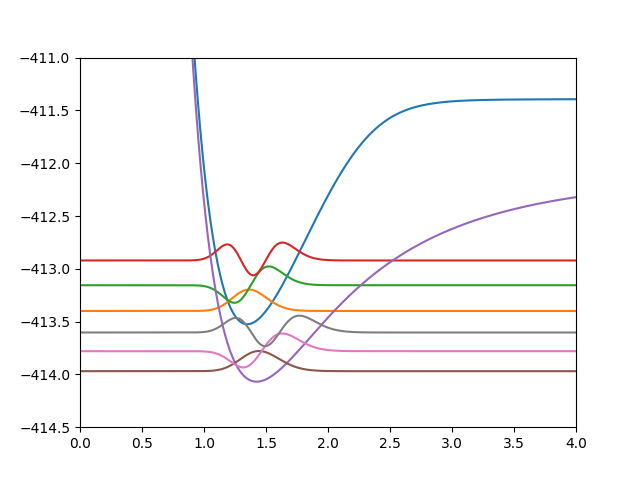
\includegraphics[width=0.8\textwidth]{../img/VibrStavy1.png}
\caption{Nejnižší vibrační hladiny molekul $\mathrm{BeH/BeH^-}$}
\label{Vibr1}
\end{figure}


\centering
\label{TODO}
\begin{tabular}{rrrrr}
\toprule
Method & $E_a(BeH)[" eV"]$ & $E_a(H)[" eV"]$ & $D_a(BeH)[" eV"]$ & $D_a(BeH^-)[" eV"]$ \\ \midrule
    Experimental:  & $0.70\pm0.1$ & $0.754195$        & $2.18\pm0.02$ & $2.07$ \\ \midrule
FCI  /aug-cc-pVDZ & 0.542 & 0.679 & 1.895 & 1.759\\
RCCSD(T)  /aug-cc-pVDZ & 0.534 & 0.679 & 1.888 & 1.744\\
CI 5,1,1,0 /aug-cc-pVDZ & 0.536 & -0.325 & 1.892 & 2.753\\
CI 6,2,2,0 /aug-cc-pVDZ & 0.542 & 0.678 & 1.893 & 1.756\\
FCI  /aug-cc-pCVDZ & 0.546 & 0.679 & 1.901 & 1.769\\
RCCSD(T)  /aug-cc-pCVDZ & 0.538 & 0.679 & 1.894 & 1.753\\
CI 5,1,1,0 /aug-cc-pCVDZ & 0.540 & 0.603 & 1.898 & 1.835\\
CI 6,2,2,0 /aug-cc-pCVDZ & 0.528 & 0.670 & 1.899 & 1.756\\
FCI  /cc-pVTZ & 0.326 & -0.091 & 1.990 & 2.407\\
RCCSD(T)  /cc-pVTZ & 0.320 & -0.091 & 1.983 & 2.394\\
CI 6,2,2,0 /cc-pVTZ & 0.325 & -0.091 & 1.988 & 2.404\\
FCI  /aug-cc-pVTZ & 0.570 & 0.734 & 2.010 & 1.847\\
RCCSD(T)  /aug-cc-pVTZ & 0.562 & 0.734 & 2.003 & 1.832\\
CI 6,2,2,0 /aug-cc-pVTZ & 0.569 & 0.732 & 2.006 & 1.844\\
RCCSD(T)  /aug-cc-pVQZ & 0.566 & 0.746 & 2.034 & 1.854\\
CI 5,1,1,0 /aug-cc-pVQZ & 0.565 & 0.744 & 2.038 & 1.858\\
CI 6,2,2,0 /aug-cc-pVQZ & 0.572 & 0.746 & 2.039 & 1.865\\
CI 9,3,3,1 /aug-cc-pVQZ & 0.573 & 0.746 & 2.039 & 1.867\\
CI 5,1,1,0 /aug-cc-pV5Z & 0.567 & 0.750 & 2.044 & 1.862\\
CI 6,2,2,0 /aug-cc-pV5Z & 0.575 & 0.752 & 2.046 & 1.869\\
\bottomrule
\end{tabular}

    
\begin{tabular}{rrrrr}
\toprule
Method & $v_0 [\mathrm{eV}]$ & $v_1 [\mathrm{eV}]$ & $v_2 [\mathrm{eV}]$ & $v_3[\mathrm{eV}]$ \\ \midrule
    FCI  /aug-cc-pVDZ & 0.1240 & 0.3648 & 0.5953 & 0.8152\\
RCCSD(T)  /aug-cc-pVDZ & 0.1244 & 0.3661 & 0.5975 & 0.8186\\
CI 5,1,1,0 /aug-cc-pVDZ & 0.1240 & 0.3649 & 0.5954 & 0.8153\\
CI 6,2,2,0 /aug-cc-pVDZ & 0.1240 & 0.3648 & 0.5953 & 0.8152\\
FCI  /aug-cc-pCVDZ & 0.1245 & 0.3658 & 0.5966 & 0.8168\\
RCCSD(T)  /aug-cc-pCVDZ & 0.1249 & 0.3670 & 0.5988 & 0.8201\\
CI 5,1,1,0 /aug-cc-pCVDZ & 0.1245 & 0.3658 & 0.5967 & 0.8169\\
CI 6,2,2,0 /aug-cc-pCVDZ & 0.1245 & 0.3658 & 0.5966 & 0.8168\\
FCI  /cc-pVTZ & 0.1254 & 0.3688 & 0.6021 & 0.8252\\
RCCSD(T)  /cc-pVTZ & 0.1257 & 0.3698 & 0.6039 & 0.8281\\
CI 6,2,2,0 /cc-pVTZ & 0.1254 & 0.3688 & 0.6021 & 0.8252\\
FCI  /aug-cc-pVTZ & 0.1252 & 0.3682 & 0.6010 & 0.8234\\
RCCSD(T)  /aug-cc-pVTZ & 0.1255 & 0.3692 & 0.6028 & 0.8263\\
CI 6,2,2,0 /aug-cc-pVTZ & 0.1254 & 0.3691 & 0.6032 & 0.8275\\
RCCSD(T)  /aug-cc-pVQZ & 0.1261 & 0.3713 & 0.6065 & 0.8314\\
CI 5,1,1,0 /aug-cc-pVQZ & 0.1258 & 0.3704 & 0.6047 & 0.8287\\
CI 6,2,2,0 /aug-cc-pVQZ & 0.1258 & 0.3704 & 0.6047 & 0.8286\\
CI 9,3,3,1 /aug-cc-pVQZ & 0.1258 & 0.3704 & 0.6047 & 0.8286\\
CI 5,1,1,0 /aug-cc-pV5Z & 0.1259 & 0.3707 & 0.6052 & 0.8293\\
CI 6,2,2,0 /aug-cc-pV5Z & 0.1259 & 0.3707 & 0.6052 & 0.8293\\
\bottomrule
\end{tabular}
    
\label{TODO}
\begin{tabular}{rrrrr}
\toprule
Method & $E_a(OH)[" eV"]$ & $E_a(O)[" eV"]$ & $D_a(OH)[" eV"]$ & $D_a(OH^-)[" eV"]$ \\ \midrule
Experimental:  & $1.82767$ & $1.461$ &        $4.3914$ & $5.120435$ \\ \midrule
CI 4,1,1,0 /aug-cc-pVDZ & 1.345 & -1.637 & 4.054 & 7.035\\
CI 4,2,2,0 /aug-cc-pVDZ & 1.559 & 1.084 & 4.090 & 4.565\\
CI 6,2,2,0 /aug-cc-pVDZ & 1.609 & 1.182 & 4.104 & 4.531\\
CI 8,2,2,0 /aug-cc-pVDZ & 1.614 & 1.188 & 4.101 & 4.527\\
CI 4,1,1,0 /aug-cc-pVTZ & 1.376 & -1.517 & 4.234 & 7.127\\
CI 4,2,2,0 /aug-cc-pVTZ & 1.629 & 1.158 & 4.269 & 4.739\\
CI 6,2,2,0 /aug-cc-pVTZ & 1.687 & 1.303 & 4.306 & 4.690\\
CI 8,2,2,0 /aug-cc-pVTZ & 1.693 & 1.308 & 4.296 & 4.681\\
CI 4,1,1,0 /aug-cc-pVQZ & 1.413 & -1.480 & 4.292 & 7.185\\
CI 4,2,2,0 /aug-cc-pVQZ & 1.674 & 1.218 & 4.332 & 4.789\\
CI 6,2,2,0 /aug-cc-pVQZ & 1.733 & 1.362 & 4.369 & 4.740\\
CI 8,2,2,0 /aug-cc-pVQZ & 1.740 & 1.368 & 4.359 & 4.730\\
\bottomrule
\end{tabular}
    
\begin{table}[]
\centering
\caption{OH vibration states}
\label{TODO}
\begin{tabular}{rrrrr}
\toprule
Method & $v_0 [" eV"]$ & $v_1 [" eV"]$ & $v_2 [" eV"]$ & $v_3[" eV"]$ \\ \midrule
CI 4,1,1,0 /aug-cc-pVDZ & 0.225 & 0.657 & 1.065 & 1.451\\
CI 4,2,2,0 /aug-cc-pVDZ & 0.224 & 0.656 & 1.063 & 1.448\\
CI 6,2,2,0 /aug-cc-pVDZ & 0.224 & 0.656 & 1.064 & 1.450\\
CI 8,2,2,0 /aug-cc-pVDZ & 0.224 & 0.656 & 1.063 & 1.449\\
CI 4,1,1,0 /aug-cc-pVTZ & 0.227 & 0.665 & 1.081 & 1.474\\
CI 4,2,2,0 /aug-cc-pVTZ & 0.227 & 0.664 & 1.078 & 1.469\\
CI 6,2,2,0 /aug-cc-pVTZ & 0.227 & 0.664 & 1.079 & 1.473\\
CI 8,2,2,0 /aug-cc-pVTZ & 0.227 & 0.664 & 1.078 & 1.471\\
CI 4,1,1,0 /aug-cc-pVQZ & 0.228 & 0.668 & 1.085 & 1.481\\
CI 4,2,2,0 /aug-cc-pVQZ & 0.227 & 0.665 & 1.080 & 1.474\\
CI 6,2,2,0 /aug-cc-pVQZ & 0.227 & 0.667 & 1.084 & 1.479\\
CI 8,2,2,0 /aug-cc-pVQZ & 0.227 & 0.666 & 1.083 & 1.477\\
\bottomrule
\end{tabular}
\end{table}
    
\begin{tabular}{rrrrr}
\toprule
Method & $v_0 [\mathrm{eV}]$ & $v_1 [\mathrm{eV}]$ & $v_2 [\mathrm{eV}]$ & $v_3[\mathrm{eV}]$ \\ \midrule
CI 4,1,1,0 /aug-cc-pVDZ & 0.228 & 0.662 & 1.069 & 1.449\\
CI 4,2,2,0 /aug-cc-pVDZ & 0.221 & 0.647 & 1.047 & 1.426\\
CI 6,2,2,0 /aug-cc-pVDZ & 0.224 & 0.655 & 1.059 & 1.440\\
CI 8,2,2,0 /aug-cc-pVDZ & 0.224 & 0.653 & 1.057 & 1.437\\
CI 4,1,1,0 /aug-cc-pVTZ & 0.212 & 0.637 & 1.047 & 1.448\\
CI 4,2,2,0 /aug-cc-pVTZ & 0.221 & 0.649 & 1.054 & 1.439\\
CI 6,2,2,0 /aug-cc-pVTZ & 0.225 & 0.661 & 1.072 & 1.460\\
CI 8,2,2,0 /aug-cc-pVTZ & 0.225 & 0.660 & 1.070 & 1.457\\
CI 4,1,1,0 /aug-cc-pVQZ & 0.212 & 0.637 & 1.052 & 1.455\\
CI 4,2,2,0 /aug-cc-pVQZ & 0.224 & 0.657 & 1.066 & 1.450\\
CI 6,2,2,0 /aug-cc-pVQZ & 0.225 & 0.663 & 1.077 & 1.467\\
CI 8,2,2,0 /aug-cc-pVQZ & 0.225 & 0.662 & 1.075 & 1.463\\
\bottomrule
\end{tabular}
    
%\include{kap03}
%\include{kap04}

\chapter*{Závěr}
\addcontentsline{toc}{chapter}{Závěr}
Pro dvě molekuly, BeH a OH, jsme získali křivky excitovaných stavů molekuly pro použití v 
R-maticových výpočtech i referenční křivky pro nastavení parametrů těchto výpočtů.
Pro molekulu BeH jsme při referenčních výpočtech metodou MRCI získali křivky dostatečně 
přesné pro nastavení R-maticových výpočtů. Pro popis excitovaných stavů neutrální 
molekuly BeH pro R-maticové výpočty pak navrhujeme použít metodu CAS-SCF s aktivním 
prostorem 6,2,2,0 v aug-cc-pVDZ bázi. Pro popis excitovaných stavů molekuly BeH je 
dle našich zjištění nutné používat augmented báze.

Pro molekulu OH jsme metodou MRCI v aug-cc-pV5Z získali křivky konzistentní s
experimentálními daty, které lze použít pro nastavení R-maticových výpočtů.
Zároveň jsme nalezli vhodný popis excitovaných stavů pomocí metod CAS-SCF s aktivními
prostory 6,2,2,0 a 7,3,3,0 v aug-cc-pVDZ, spolu s vhodným nalezením vah jednotlivých 
stavů vylepšující konverenci stavů, které navrhujeme pro použití v R-maticových 
výpočtech. Augmentované báze se ukázaly být lepší v popisu excitovaných stavů této 
molekuly, ačkoliv rozdíl nebyl tak zásadní jako u molekuly BeH.

Na těchto výsledcích budou dále prováděny R-maticové výpočty, které nebyly z časových důvodů zahrnuty již do této práce.

%%% Seznam použité literatury
%%% Seznam použité literatury (bibliografie)
%%%
%%% Pro vytváření bibliografie používáme bibTeX. Ten zpracovává
%%% citace v textu (např. makro \cite{...}) a vyhledává k nim literaturu
%%% v souboru literatura.bib.
%%%
%%% Příkaz \bibliographystyle určuje, jakým stylem budou citovány odkazy
%%% v textu. V závorce je název zvoleného souboru .bst. Styly plainnat
%%% a unsrt jsou standardní součástí latexových distribucí. Styl czplainnat
%%% je dodáván s touto šablonou a bibTeX ho hledá v aktuálním adresáři.

%\bibliographystyle{czplainnat}    %% Autor (rok) s českými spojkami
%\bibliographystyle{plainnat}    %% Autor (rok) s anglickými spojkami
\bibliographystyle{unsrt}       %% [číslo]

\renewcommand{\bibname}{Seznam použité literatury}

%%% Vytvoření seznamu literatury. Pozor, pokud jste necitovali ani jednu
%%% položku, seznam se automaticky vynechá.

\bibliography{literatura}

%%% Kdybyste chtěli bibliografii vytvářet ručně (bez bibTeXu), lze to udělat
%%% následovně. V takovém případě se řiďte normou ISO 690 a zvyklostmi v oboru.

% \begin{thebibliography}{99}
%
% \bibitem{lamport94}
%   {\sc Lamport,} Leslie.
%   \emph{\LaTeX: A Document Preparation System}.
%   2. vydání.
%   Massachusetts: Addison Wesley, 1994.
%   ISBN 0-201-52983-1.
%
% \end{thebibliography}


%%% Obrázky v bakalářské práci
%%% (pokud jich je malé množství, obvykle není třeba seznam uvádět)
\listoffigures

%%% Tabulky v bakalářské práci (opět nemusí být nutné uvádět)
%%% U matematických prací může být lepší přemístit seznam tabulek na začátek práce.
\listoftables

%%% Použité zkratky v bakalářské práci (opět nemusí být nutné uvádět)
%%% U matematických prací může být lepší přemístit seznam zkratek na začátek práce.
%\chapwithtoc{Seznam použitých zkratek}

%%% Přílohy k bakalářské práci, existují-li. Každá příloha musí být alespoň jednou
%%% odkazována z vlastního textu práce. Přílohy se číslují.
%%%
%%% Do tištěné verze se spíše hodí přílohy, které lze číst a prohlížet (dodatečné
%%% tabulky a grafy, různé textové doplňky, ukázky výstupů z počítačových programů,
%%% apod.). Do elektronické verze se hodí přílohy, které budou spíše používány
%%% v elektronické podobě než čteny (zdrojové kódy programů, datové soubory,
%%% interaktivní grafy apod.). Elektronické přílohy se nahrávají do SISu a lze
%%% je také do práce vložit na CD/DVD. Povolené formáty souborů specifikuje
%%% opatření rektora č. 72/2017.
\appendix
%\chapter{Přílohy}

%\section{První příloha}

\openright
\end{document}
